
\chapter{Systeem overzicht en ontwerp}
Het systeem is opgedeeld in vier blokken:
\begin{itemize}
\item De DCF controller
\item De main controller
\item Het alarm
\item De LCD controller
\end{itemize}

\noindent In figuur \ref{fig:blokdiagram} is te zien welke ingangs- en uitgangssignalen het systeem in en uit gaan en hoe de blokken elkaar aansturen.

\begin{figure}[h!]
\center
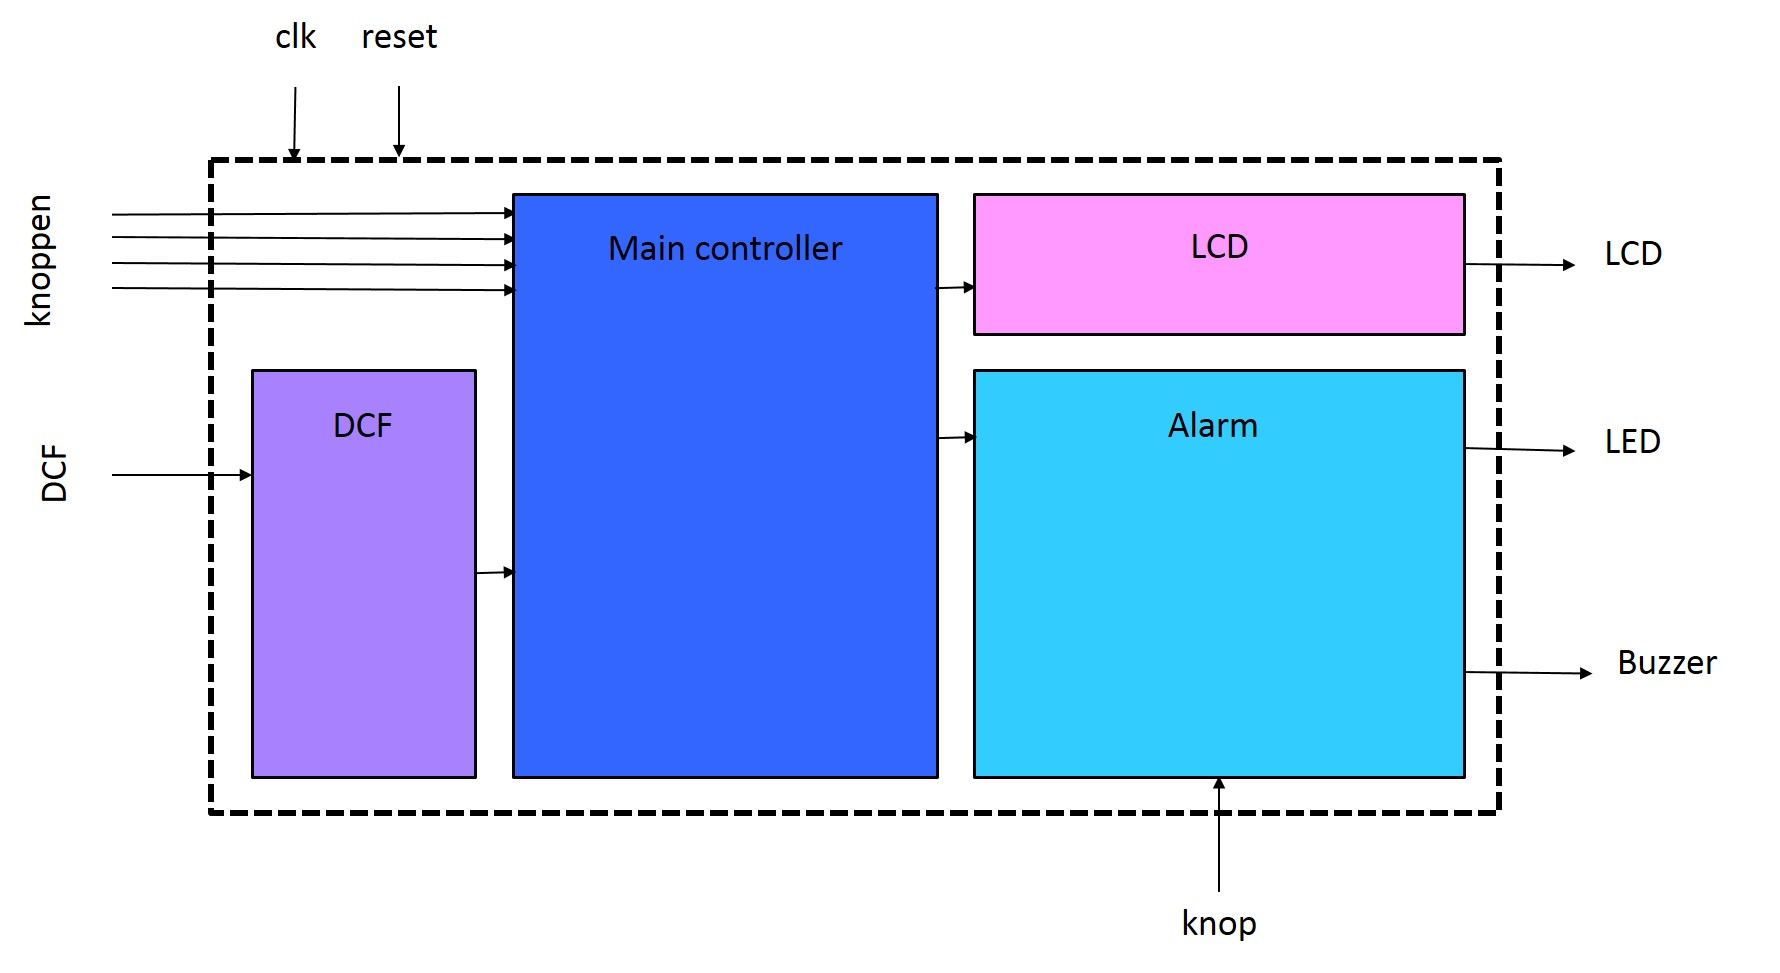
\includegraphics[width=15cm]{figure/blokdiagram}
\caption{Blokdiagram van het gehele systeem}
\label{fig:blokdiagram}
\end{figure}

\noindent De DCF controller vangt het DCF signaal op en zet het om naar een bitvector met datum, uren en minuten. En er wordt een kloksignaal van 1 Hz gegenereerd. Mocht het DCF-signaal tijdelijk niet goed opgevangen kunnen worden, kan een intern register de tijd door blijven geven en er gaat een ledje branden om aan te geven dat de chip geen DCF-signaal meer ontvangt. Dit register wordt dan weer gesynchroniseerd als het signaal weer opgevangen wordt.\\
De main controller bestuurt het hele systeem. De alarmtijd kan ingesteld worden en de alarmtijd wordt met de actuele tijd vergeleken, zodat het alarmblok weet wanneer het alarm aan moet gaan. Met knoppen kan het menu bestuurd worden.\\
In het alarmblok wordt eerst de vijftien minuten van de wekkertijd afgetrokken. De ingestelde tijd is namelijk de tijd waarop het geluid aan moet gaan, de lamp moet al een kwartier eerder beginnen met branden. Daarnaast zorgt het alarm ervoor dat een PWM-signaal gegenereerd wordt wat naar een LED gaat. \\
De LCD controller zorgt dat de datum, tijd, ingestelde alarmtijd en de veranderingen in het menu op de LCD zichtbaar zijn. Er wordt een LCD scherm gebruikt waar de pixels afzonderlijk van elkaar aangestuurd worden. Tussen de chip en het scherm zit nog een microcontroller, waarin de karakters zijn opgeslagen, dit zou namelijk te groot zijn om op de chip te regelen.
